\documentclass{beamer}
\usepackage{listings}
\lstset{
%language=C,
frame=single, 
breaklines=true,
columns=fullflexible
}
\usepackage{subcaption}
\usepackage{url}
\usepackage{tikz}
\usepackage{graphicx}
\usepackage{tkz-euclide} % loads  TikZ and tkz-base
%\usetkzobj{all}
\usetikzlibrary{calc,math}
\usepackage{float}
\newcommand\norm[1]{\left\lVert#1\right\rVert}
\renewcommand{\vec}[1]{\mathbf{#1}}
\newcommand{\R}{\mathbb{R}}
\newcommand{\C}{\mathbb{C}}
\providecommand{\brak}[1]{\ensuremath{\left(#1\right)}}
\providecommand{\abs}[1]{\vert#1\vert}
\providecommand{\fourier}{\overset{\mathcal{F}}{ \rightleftharpoons}}
\providecommand{\pr}[1]{\ensuremath{\Pr\left(#1\right)}}
\providecommand{\sbrak}[1]{\ensuremath{{}\left[#1\right]}}
\usepackage[export]{adjustbox}
\usepackage[utf8]{inputenc}
\usepackage{amsmath}
\usetheme{Boadilla}
\title{Markov Chains}
\author{Taha Adeel Mohammed}
\institute{IITH(CSE)}
\date{\today}
\begin{document}
%
\begin{frame}
\titlepage
\end{frame}
\begin{frame}{Prerequisites}
%\frametitle{Prerequisites}
\begin{block}{State Space}
The set of all possible states the system/object can be in. Without loss in generality, the state space can be identified with the set $S=\{ 1,2,\dots,\ell\}$, where $\ell$ is a fixed arbitrary natural number.
\end{block}
\begin{block}{Random variables}
%Furthermore, for each pair $ i,j\in S$ we consider the (conditional) probability $ p_{ij}\in[0,1]$ for the transition of the object or system from state $ i$ to $ j$ within one time step.
Let $\{ X_0,X_1,X_2\dots\}$ be a sequence of discrete random variables, where each $X_t \in S$, and $X_t$ represents the state of the system at time $t$.
\end{block}
\end{frame}
\begin{frame}{Definition}
\begin{itemize}
    \item A process is said to be a Markov Process if the probability of transitioning to any particular state is dependent solely on the current state and does not depend on how the current state was reached.
    \item Mathematically, $ \{X_0,X_1,\ldots\}$ is called a  Markov chain if 
\begin{align}
    \pr{(X_{n}=i_n\mid X_{n-1}=i_{n-1},\ldots,X_0=i_{0}}= \pr{X_{n}=i_n\mid X_{n-1}=i_{n-1}}
\end{align}
\item This is known as the Markov property
\end{itemize}
\end{frame}
\begin{frame}{Transition matrix}
    \begin{block}{Transition matrix}
    \begin{itemize}
        \item  For each pair $ i,j\in S$, consider the (conditional) probability $ p_{ij}\in[0,1]$ for the transition of the object or system from state $ i$ to $ j$ within one time step.
        \item The $ \ell\times\ell$ matrix $ {\mathbf{P}}=(p_{ij})_{i,j=1,\ldots,\ell}$ of the transition probabilities $ p_{ij}$ where
        \begin{align}
            p_{ij}\ge0\,,\qquad p_{ij}=\pr{X_{n+1}=j\mid X_{n}=i}	
        \end{align}
        is called one-step \textit{transition matrix} or simply transition matrix of the Markov chain.
    \end{itemize}
    \end{block}
\end{frame}
\begin{frame}{Transition matrix(contd.)}
    \begin{theorem}
    Let $\{X_0, X_1, X_2, . . .\}$ be a Markov chain with a $\ell \times \ell $ transition matrix $P$. Then the 2-step transition probabilities are given by the matrix $P^2$. That is,
    \begin{align}
        \pr{X_{n+2}=j\mid X_{n}=i}	= (P^2)_{ij}
    \end{align}
    \end{theorem}
    \begin{proof}
    \begin{itemize}
        \item Recall matrix multiplication. Let $A = (a_{ij} )$ and $B = (b_{ij})$ be $N \times N$ matrices.The product matrix is $A \times B = AB$, with elements
        \begin{align}
            (AB)_{ij}= \sum\limits_{k=0}^N a_{ik}b_{kj}
        \end{align}
        \end{itemize}
    \end{proof}
\end{frame}
\begin{frame}{}
    \begin{proof}[Proof(Contd.)]
        \vspace{-5mm}
        \begin{align}
            \pr{X_{2}=j | X_0=i}&=\sum\limits_{k=0}^\ell \pr{X_{2}=j | X_{1}=k, X_0=i}\pr{X_{1}=k | X_0=i}\\
            &=\sum\limits_{k=0}^\ell \pr{X_{2}=j | X_{1}=k}\pr{X_{1}=k | X_0=i}\\
            &=\sum\limits_{k=0}^\ell p_{kj}p_{ik}\\
            &=\sum\limits_{k=0}^\ell p_{ik}p_{kj}       =(P^2)_{ij}\\
            \pr{X_{2}=j | X_0=i}&=\pr{X_{n+2}=j | X_n=i}=(P^2)_{ij}
        \end{align}
        \vspace{-8mm}
        \begin{itemize}
            \item Similarly it can be proved that the $t$-step transition matrix is equal to $P^t$.
        \end{itemize}
    \end{proof}
\end{frame}
\begin{frame}{Example question}
\begin{block}{Problem (GATE 2008 (CS), Q.27)}
Aishwarya studies either computer science or mathematics everyday. If she studies computer science on a day, then the probability she studies mathematics the next day is 0.6. If she studies mathematics on a day, then the probability she studies computer science the next day is 0.4.
Given that Aishwarya studies computer science on Monday, what is the probablity she studies computer science on Wednesday?
\begin{enumerate}
%\setlength\itemsep{2em}
\item 0.24
\item 0.36
\item 0.4
\item 0.6
\end{enumerate}
\end{block}    
\end{frame}
\begin{frame}{Solution}
\begin{block}{State space}
Consider the state space $S=\{1,2\}$, where $1$ represents Aishwarya studying CS and $2$ represents her studying maths on a particular day.
\end{block}
\begin{block}{Markov chain}
Let $\{X_0, X_1, \dots\}$ be a series of random variables(which form a Markov chain) where $X_i \in S$ represents her studying CS or maths on the $i$th day(i=0 for Monday)
\end{block}
\end{frame}
\begin{frame}{Solution}
\begin{block}{Transition matrix}
The one step state transition matrix $P=(p_{ij})$ for the markov chain (where $p_{ij}=\pr{X_{n+1}=j\, |\, X_{n}=i}$) is :-
\begin{align}
\,\,\overbrace{
 \begin{matrix}
1 & \,\,\,\,\,\,2
\end{matrix}\nonumber}^{X_{n+1}}\nonumber
\end{align}
\vspace{-1cm}
\begin{align}
P\,\,=\,\,\,\,\scriptstyle{X_n\,\,} \bigg\{ \, \begin{matrix} 1\\ 2 \end{matrix}\,\,\,
 \begin{bmatrix}
x & 0.6 \\
0.4 & y 
\end{bmatrix}\,\,=\,\,
\begin{bmatrix}
0.4 & 0.6 \\
0.4 & 0.6 
\end{bmatrix}
\end{align}
\end{block}
As $X_n=1 \text{ and } X_n=2$ are mutually exclusive, we can easily calculate $x$ and $y$.
\begin{align}
   x=\pr{X_{n+1} = 1 |\, X_{n}=2} &= 1-\pr{X_{n+1} = 2 \,| X_{n}=1}\nonumber
    \\&= 0.4 \label{x}\\
    y=\pr{X_{n+1} = 2 |\, X_{n}=2} &= 1-\pr{X_{n+1} = 1 \,| X_{n}=2}\nonumber
    \\&= 0.6 \label{y}
\end{align}
\end{frame}

\begin{frame}{Solution}
\begin{figure}[h]
    \centering
     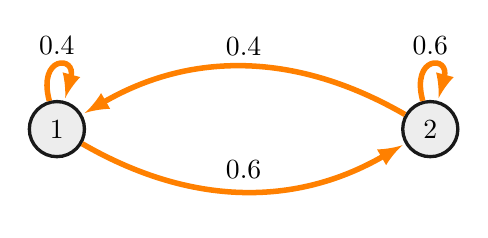
\begin{tikzpicture}[
roundnode/.style={circle, draw=black!90, fill=black!7, very thick, minimum size=7mm},
]
%Nodes
\node[roundnode]        (Computer_Science)        {1};
\node[roundnode]        (Mathematics)       [right=4cm of Computer_Science] {2};
%Lines
 \draw[every loop,
        auto=right,
        line width=0.7mm,
        >=latex,
        draw=orange,
        fill=orange]
            (Computer_Science) edge[bend right, auto=left]  node {0.6} (Mathematics)
            (Mathematics) edge[bend right, auto=right] node {0.4} (Computer_Science)
            (Computer_Science) edge[loop above]             node {0.4} (Computer_Science)
            (Mathematics) edge[loop above]             node {0.6} (Mathematics);
\end{tikzpicture}
    \caption{Markov Diagram}
\end{figure}
\end{frame}
\begin{frame}{Solution}
\begin{itemize}
    \item     Given that her initial state is $X_0=1$ ($\because$ she studies CS on Monday(n=0)).
    \item The $\pr{X_{n+2}=j \, |\, X_{n}=i}$ is given by the $(i,j)$th position of $P^{\,2}$.
    \item Therefore $\pr{X_{2}=1 | X_{0}=1}$ ($\because$ n=2 for Wednesday) is the $(1,1)$th position of $P^2$.
\begin{align}
    P^2=\begin{bmatrix}
0.4 & 0.6 \\
0.4 & 0.6
\end{bmatrix}\times
\begin{bmatrix}
0.4 & 0.6 \\
0.4 & 0.6 
\end{bmatrix}=
\begin{bmatrix}
0.4 & 0.6 \\
0.4 & 0.6 
\end{bmatrix}
\end{align}
\item $\therefore$ The probability she studies computer science on Wednesday is $(P^{2})_{1\,1} = 0.4$.\\
(\textbf{Ans: Option (3)})
\end{itemize}
\end{frame}
\end{document}
